%
% Emulating Enigma
% (C) 2015 Manolis Kiagias
% Published under the Creative Commons license 
%
%!TEX TS-program = xelatex
%!TEX encoding = UTF-8 Unicode
%
\documentclass[a4paper,twoside,12pt]{article}
\usepackage{fontspec,xltxtra,xunicode}
% Begin new paragraphs with an empty line rather than an indent
\usepackage[parfill]{parskip}
\usepackage{xgreek}
\usepackage{multirow}
\usepackage{longtable}
\usepackage{tabularx}
\usepackage{xcolor}
\usepackage{minted}
\usepackage{enumitem}
\usepackage[colorlinks=true,linkcolor=black]{hyperref}
\defaultfontfeatures{Mapping=tex-text}
\setromanfont[Mapping=tex-text]{Times New Roman}
\setsansfont[Scale=MatchLowercase,Mapping=tex-text]{Liberation Sans}
\setmonofont[Scale=MatchLowercase]{Liberation Mono}
\setmainfont[Scale=MatchLowercase]{Liberation Serif}
\usepackage{multicol}
\usepackage{graphicx}
\setcounter{secnumdepth}{4}
\setcounter{tocdepth}{4}
\usepackage{fancyhdr}
\pagestyle{fancy}
\renewcommand{\sectionmark}[1]{%
	\markboth{#1}{}}
\fancyhf{}
\fancyhead[LE,RO]{\bfseries\thepage}
\fancyhead[LO]{\bfseries\rightmark}
\fancyhead[RE]{\bfseries\leftmark}
\renewcommand{\headrulewidth}{0.5pt}
\renewcommand{\footrulewidth}{0pt}
\addtolength{\headheight}{0.5pt}
\fancypagestyle{plain}{%
	\fancyhead{}
	\renewcommand{\headrulewidth}{0pt}}
%
% User defined environments and commands
%
\newenvironment{inthebox}{\line(1,0){390}\\}%
{\line(1,0){390}}
\newcommand{\coderoot}[1]{\texttt{\# #1}}
\newcommand{\codeuser}[1]{\texttt{\$ #1}}
\newcommand{\code}[1]{\texttt{#1}}
\definecolor {bg} {rgb}{1.00, 1.00, 1.00}
\setlist[description]{style=nextline}

%
% Title page
%
\author{Μανώλης Κιαγιάς, MSc}
\title {Εξομοιώνοντας την Enigma}
\date{17/11/2015}
%
%
\begin{document}
%
\maketitle
%
\cleardoublepage
%
%
% Book intro pages (frontmatter)
%
\begin{center}
Copyright \copyright 2015 Μανώλης Κιαγιάς\\
Το Παρόν Έργο παρέχεται υπό τους όρους της Άδειας:\\

\includegraphics[scale=0.2]{images/license/cc-logo}\\
\textbf{Αναφορά Δημιουργού-Μη Εμπορική Χρήση-Παρόμοια Διανομή 4.0 Διεθνής}\\
Το πλήρες κείμενο αυτής της άδειας είναι διαθέσιμο εδώ:\\
\url{http://creativecommons.org/licenses/by-nc-sa/4.0/}
\end{center}
\subsection*{Είστε ελεύθερος να:}
\noindent
\textbf{Διαμοιραστείτε} -- να αντιγράψετε και αναδιανείμετε το υλικό με οποιοδήπότε μέσο και μορφή.\\
\textbf{Προσαρμόσετε} -- να αναμείξετε, μετασχηματίσετε και να επεκτείνετε το υλικό.\\

Ο αδειοδότης δεν μπορεί να σας αφαιρέσει αυτές τις ελευθερίες όσο ακολουθείτε τους όρους της παρούσας άδειας.
\subsection*{Ύπο τους ακόλουθους όρους:}

\vspace{1em}
\noindent
\parbox{1.5cm}{
\includegraphics[scale=0.15]{images/license/cc_by_30}}
\parbox{10.5cm}{\textbf{Αναφορά Δημιουργού} -- Θα πρέπει να αναφέρετε \textbf{τον δημιουργό του έργου}, να παρέχετε σύνδεσμο προς αυτή την άδεια, και να \textbf{υποδείξετε τυχόν αλλαγές}. Μπορείτε να το κάνετε με οποιοδήποτε εύλογο μέσο, αλλά όχι με τρόπο που να υπονοεί ότι ο αδειοδότης επικροτεί εσάς ή τη χρήση του έργου από εσάς.}

\vspace{1em}
\noindent
\parbox{1.5cm}{
\includegraphics[scale=0.15]{images/license/cc_nc_30}}
\parbox{10.5cm}{\textbf{Μη Εμπορική Χρήση} --  Δεν μπορείτε να χρησιμοποιήσετε το υλικό για \textbf{εμπορικούς σκοπούς}.}

\vspace{1em}
\noindent
\parbox{1.5cm}{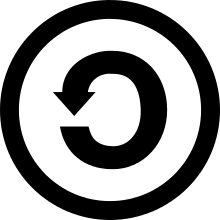
\includegraphics[scale=0.15]{images/license/cc_sa_30}}
\parbox{10.5cm}{\textbf{Παρόμοια Διανομή}  -- Αν αναμείξετε, μετασχηματίσετε ή επεκτείνετε το υλικό, θα πρέπει να διανείμετε τις αλλαγές σας υπό την \textbf{ίδια άδεια} με το πρωτότυπο έργο.}

\vspace{1em}
\noindent
\parbox{1.5cm}{\ }
\parbox{10.5cm}{\textbf{Όχι επιπλέον περιορισμοί} -- Δεν μπορείτε να εφαρμόσετε νομικούς όρους ή \textbf{τεχνικά μέσα} που να περιορίζουν νομικά τους άλλους να πράξουν σύμφωνα με τις ελευθερίες αυτής της άδειας.}
\subsection*{Σημειώσεις:}
\noindent
Δεν χρειάζεται να ακολουθήσετε την άδεια για τμήματα του υλικού που θεωρούνται δημόσια γνώση (public domain) ή όπου η χρήση τους επιτρέπεται εξαιτίας μιας \textbf{εξαίρεσης ή περιορισμού}.\\

\noindent
Δεν δίνονται εγγυήσεις. Η άδεια ίσως να μη σας δίνει όλα τα δικαιώματα για την επιδιωκόμενη χρήση. Για παράδειγμα, επιπλέον δικαιώματα όπως \textbf{δημοσιότητα, ιδιωτικότητα, ή ηθικά δικαιώματα} μπορεί να επιβάλλουν περιορισμούς στη χρήση του υλικού.\\
\line(1,0){390}\\\\
\noindent
Το παρόν έργο στοιχειοθετήθηκε σε \XeLaTeX. Ο πηγαίος κώδικας του είναι διαθέσιμος στην παρακάτω τοποθεσία:
\begin{center}
\url{http://www.github.com/sonic2000gr/enigma-notes}
\end{center}
\newpage
\tableofcontents
\newpage

%
\section{Εισαγωγή στην Κρυπτογραφία}
%
Σε μια εποχή που οι υπολογιστές δεν είχαν ακόμα κάνει την εμφάνιση τους, πριν ακόμα και από τον πρώτο ηλεκτρονικό υπολογιστή (Eniac), μια μηχανή κρυπτογράφησης έθετε σε κίνδυνο την έκβαση του 2ου Παγκοσμίου Πολέμου: Βλέπετε, η μηχανή Enigma, μια εκπληκτική ηλεκτρομηχανική κατασκευή κρυπτογράφησης / αποκρυπτογράφησης, άνηκε στους Γερμανούς και χρησιμοποιούνταν για απόρρητη επικοινωνία των αρχηγείων με μονάδες στρατού και κυρίως υποβρύχια. Οι Γερμανοί τη θεωρούσαν απαραβίαστη – αλλά ευτυχώς για όλους μας, έκαναν λάθος.

Στην κρυπτογράφηση όπως και σε άλλα θέματα ασφαλείας των υπολογιστών, ισχύει η αρχή ``man make, man break'' (άνθρωπος τα φτιάχνει, άνθρωπος τα σπάει). Και αν ακόμα και σήμερα, με τα τεράστια κλειδιά μας, τους αλγόριθμους κρυπτογράφησης ανοικτού κώδικα (που τους ελέγχουν χιλιάδες μάτια), βρίσκουμε συνέχεια κενά ασφαλείας, φανταστείτε μια μηχανή που ουσιαστικά αποτελεί την έκδοση 1.0 της σύγχρονης κρυπτογραφίας: η υπερβολική εμπιστοσύνη στις ικανότητες της βλάπτει σοβαρά τα μυστικά μας!

Ο σκοπός κάθε μηχανής ή αλγόριθμου κρυπτογράφησης είναι πολύ απλός: να πάρει ένα μήνυμα (στην προκειμένη περίπτωση ένα απλό κείμενο (plaintext) που αποτελείται μόνο από τα 26 γράμματα του λατινικού αλφάβητου) και να το μετατρέψει σε ένα κρυπτόγραμμα (ciphertext), ένα κωδικοποιημένο και εντελώς ακαταλαβίστικο κείμενο που μπορεί να αποκωδικοποιηθεί μόνο από όποιον γνωρίζει κάποιο συγκεκριμένο μυστικό: ένα κωδικό, κλειδί η κάποιο συνδυασμό από αυτά. 

Η μηχανή Enigma ήταν μια ιδιαίτερα σοβαρή προσπάθεια στον τομέα αυτό, αφού όπως θα διαπιστώσετε διαβάζοντας (και βλέποντας τα σχετικά βίντεο που παραθέτουμε) είχε μια ισχύ περίπου 76bits κρυπτογράφησης, εξαιρετικά καλή για το 1940!

\subsection{Αρχές της Κρυπτογραφίας}

Το πρόβλημα της κρυπτογράφησης υπήρχε ήδη από την αρχαιότητα. Οι Σπαρτιάτες για παράδειγμα, είχαν τη σκυτάλη, μια ξύλινη ράβδο με συγκεκριμένη διάμετρο, γύρω από την οποία τύλιγαν σε ελικοειδή μορφή ένα πάπυρο. Σε αυτόν γράφονταν το αρχικό κείμενο, και όταν ξετυλίγονταν ήταν πλέον ακατάληπτο. Εκτός φυσικά αν ο παραλήπτης διέθετε μια σκυτάλη ίδιας διαμέτρου για να το ξανατυλίξει. Προφανώς το κλειδί σε αυτή την περίπτωση είναι η διάμετρος της σκυτάλης (λεπτομέρειες μπορείτε να διαβάσετε στη wikipedia: \url{http://el.wikipedia.org/wiki/Κρυπτογραφία)}.

Μια διαφορετική – αλλά εξαιρετικά ασθενής κρυπτογράφηση – είναι ο αλγόριθμος του Καίσαρα: Σε αυτόν κάθε γράμμα του αλφαβήτου μετατοπίζεται ορισμένες θέσεις μπροστά ή πίσω. Είναι εξαιρετικά εύκολο να γράψετε ένα προγραμματάκι στην αγαπημένη σας γλώσσα προγραμματισμού (εννοούμε βέβαια την Python) που να το κάνει. Μη ξεχνάμε άλλωστε ότι χάρη στον κώδικα ASCII, το A έχει τιμή 65 και αν το μετατοπίσουμε 3 θέσεις δεξιά θα γίνει 68 δηλ. D. Το μόνο που έχετε να κάνετε λοιπόν είναι να χωρίσετε το μήνυμα σας σε γράμματα και να εφαρμόσετε το παραπάνω σε κάθε γράμμα. Δείτε το πρόγραμμα \textbf{caesar.py}:

\begin{minted}[bgcolor=bg, linenos, frame=lines, framesep=10pt]{python}
#Πρόγραμμα: caesar.py
#
# Simple Caesar cipher
# (shifts 3 places to the right)
# we of course prefer Ceasar salads!
#
plaintext = raw_input("Enter text:")
plaintext = plaintext.upper()
ciphertext = ""
for letter in plaintext:
    newletter = ord(letter) + 3
    if newletter > 90:
        newletter = newletter - 26
    ciphertext = ciphertext + chr(newletter)
print ciphertext
\end{minted}

Αν στο πρόγραμμα μας δώσετε ως είσοδο τη λέξη KOLOKYTHI θα πάρετε την έξοδο NRORNBWKL. Ας το δούμε αυτό όμως λίγο καλύτερα:

\begin{center}
\begin{tabularx}{0.95\textwidth}{|*{9}{>{\centering\arraybackslash}X|}}
\hline
K&O&L&O&K&Y&T&H&I\\
\hline
N&R&O&R&N&B&W&K&L\\
\hline
\end{tabularx}
\end{center}

Παρατηρείτε κάτι; Ίδια γράμματα στο plaintext αντιστοιχούν πάντα στο ίδιο γράμμα στο κρυπτόγραμμα. Το O γίνεται πάντα R, το K γίνεται πάντα Ν. Δεν χρειάζεται καν να γράψετε ένα πρόγραμμα που να αποκωδικοποιεί δοκιμάζοντας όλες τις πιθανές μετατοπίσεις χαρακτήρων. Αρκεί να ξέρετε σε ποια γλώσσα είναι το μήνυμα. Για κάθε γλώσσα γνωρίζουμε ποιο είναι το  συχνότερα χρησιμοποιούμενο γράμμα. Π.χ. για τα Ελληνικά είναι το Α και για τα Αγγλικά το Ε.
 (διαβάστε εδώ: \url{http://el.wikipedia.org/wiki/Ανάλυση_Συχνότητας_Γλώσσας}). Με την προϋπόθεση ότι το μήνυμα μας έχει επαρκές μέγεθος, μπορούμε απλά να μετρήσουμε το γράμμα που εμφανίζεται ποιο συχνά και να βρούμε αμέσως το κλειδί! Αν δε με πιστεύετε, ορίστε ένα πρόγραμμα που μετράει τη συχνότητα γραμμάτων σε ένα αγγλικό κείμενο (\textbf{caesar-analyser.py}):
 
\begin{minted}[bgcolor=bg, linenos, frame=lines, framesep=10pt]{python}
#Πρόγραμμα: caesar-analyser.py
thetext = raw_input("Enter text:")
thetext = thetext.upper()
frequencylist = [ 0 for i in range(26)]
for letter in thetext:
    letterord = ord(letter)
    if letterord>= 65 and letterord<=90:
      letterord -= 65
      frequencylist[letterord] += 1
print frequencylist
\end{minted}

Δοκιμάστε να του δώσετε το παρακάτω σαν είσοδο:

IF THIS WORKS IT WILL PROVE THAT THE MOST COMMON LETTER USED IN THE ENGLISH LANGUAGE IS E AND IT WILL HAVE THE HIGHEST\\
FREQUENCY OF ALL THE LETTERS IN THIS MESSAGE

Και θα δείτε τον παρακάτω πίνακα συχνοτήτων:

[7, 0, 2, 2, 19, 3, 5, 11, 12, 0, 1, 10, 4, 7, 6, 1, 1, 5, 11, 16, 3, 2, 3, 0, 1, 0]

όπου το Ε εμφανίζεται 19 φορές, περισσότερο από οποιοδήποτε άλλο γράμμα. Σας προειδοποίησα!

Καθώς καταλαβαίνετε η κρυπτογράφηση του Καίσαρα είναι για (Ρωμαϊκά) πανηγύρια, ή αν προτιμάτε\ldots κολοκύθια. Αν είναι να ασχοληθείτε με κάτι που σχετίζεται με τον  Καίσαρα, προτιμήστε την αντίστοιχη\ldots σαλάτα.

Εντάξει σας ακούω να λέτε, δεν υπάρχει κάτι καλύτερο από όλα αυτά; Στο κάτω -- κάτω τόση ώρα μιλάμε για “αρχαιολογικές” κρυπτογραφήσεις. Σίγουρα θα υπάρχει κάποια απλή κρυπτογράφηση που να μη σπάει εύκολα. Ωραία, τι θα λέγατε να δοκιμάζαμε κάτι άλλο: Μια κρυπτογράφηση όπου το κλειδί δεν θα είναι ένας αριθμός αλλά μια σειρά αριθμών που θα χρησιμοποιούμε κυκλικά. Φανταστείτε δηλαδή να έχουμε συμφωνήσει στο παρακάτω κλειδί:

[ 2, 7, 3, 4, 9, 1]

Θα δουλεύαμε κάπως έτσι: Το πρώτο γράμμα θα το μετατοπίζαμε 2 θέσεις δεξιά, το επόμενο 7, το μεθεπόμενο 3 κ.ο.κ. Όταν φτάσουμε στο τέλος του κλειδιού ξαναρχίζουμε από την αρχή. Για να γίνουμε πιο\ldots μοντέρνοι, το πρόγραμμα μας δεν θα κάνει μετατοπίσεις τύπου Καίσαρα, αλλά θα χρησιμοποιεί τη συνάρτηση XOR. Τι; Δεν ξέρετε την XOR; Πρόκειται για τη λογική συνάρτηση της αποκλειστικής διάζευξης. Πάρτε ένα αριθμό, π.χ. το 65 που αντιπροσωπεύει το ASCII για το “A” και γράψτε τον στο δυαδικό:\\

65
\begin{center}
\begin{tabularx}{0.95\textwidth}{|*{8}{>{\centering\arraybackslash}X|}}
\hline
0&1&0&0&0&0&0&1\\
\hline
\end{tabularx}
\end{center}

9
\begin{center}
\begin{tabularx}{0.95\textwidth}{|*{8}{>{\centering\arraybackslash}X|}}
\hline
0&0&0&0&1&0&0&1\\
\hline
\end{tabularx}
\end{center}

\begin{minted}[bgcolor=bg, linenos, frame=lines, framesep=10pt]{python}
#Πρόγραμμα: xor.py

key = [2, 7, 3, 4, 9, 1]
keypos = 0
thetext = raw_input("Enter text:")
ciphertext = ""
for letter in thetext:
    # Bitwise XOR is '^' in Python
    ciphertext += chr(ord(letter) ^ key[keypos])
    keypos +=1
    if keypos==6:
        keypos=0
print ciphertext
\end{minted}


Αν δώσετε σαν plaintext τη λέξη KOLOKYTHI, θα πάρετε σαν αποτέλεσμα IHOKBXVOJ. Και αν δώσετε το IHOKBXVOJ σαν είσοδο, θα πάρετε τη λέξη KOLOKYTHI σαν αποτέλεσμα. Το κλειδί σας – που πρέπει να βρείτε τρόπο να στείλετε με ασφάλεια στον παραλήπτη – είναι το [2,7,3,4,9,1].

Εξακολουθούμε να έχουμε δύο προβλήματα:

\begin{itemize}
\item Το κλειδί μας είναι υπερβολικά μικρό με αποτέλεσμα ασθενική κρυπτογράφηση (καθώς επαναλαμβάνεται πολύ συχνά).
\item Δεν ξέρουμε πως να στείλουμε με ασφάλεια το κλειδί στον παραλήπτη.
\end{itemize}

Το δεύτερο πρόβλημα στην πραγματικότητα υπάρχει σε όλες τις \emph{συμμετρικές κρυπτογραφήσεις}: Συμμετρική είναι μια κρυπτογράφηση που χρησιμοποιεί το ίδιο μυστικό κλειδί για να κρυπτογραφεί και να αποκρυπτογραφεί. Προφανώς θα πρέπει να βρούμε ένα εναλλακτικό τρόπο να στείλουμε το κλειδί στον παραλήπτη και να είμαστε σίγουροι ότι δεν έχει πέσει στα χέρια κάποιου (κακόβουλου!) τρίτου προσώπου. Όλες οι κρυπτογραφήσεις που έχουμε δει μέχρι στιγμής (αλλά και το Enigma) είναι συμμετρικές.

Το πρώτο πρόβλημα μπορούμε να το λύσουμε, κάνοντας το μέγεθος του κλειδιού τουλάχιστον όσο το μέγεθος του μηνύματος! Έτσι βέβαια θα μεγιστοποιήσουμε το δεύτερο πρόβλημα, αλλά θα έχουμε μια κρυπτογράφηση που δεν σπάει! Πρόκειται για το περίφημο \emph{one time pad} (\url{https://en.wikipedia.org/wiki/One-time_pad}) για το οποίο μπορείτε να διαβάσετε θαυμάσιες ιστορίες κατασκοπίας, καθώς σε αντίθεση με πολλές άλλες κρυπτογραφήσεις μπορεί άνετα να εφαρμοστεί με μοναδικό εξοπλισμό στυλό και χαρτί!

Τώρα βέβαια – με εξαίρεση το one time pad που δεν είναι ιδιαίτερα πρακτικό για επικοινωνίες μεγάλης κλίμακας – οι άλλες κρυπτογραφήσεις  είτε δεν προσφέρουν καλή ασφάλεια είτε δεν μπορούν να εφαρμοστούν χωρίς τη βοήθεια κάποιου υπολογιστικού συστήματος, έστω και μικρής ισχύος. Ειδικά μιλώντας για τα σύγχρονα συστήματα κρυπτογράφησης – τα οποία χρησιμοποιούν\emph{ασυμμετρική κρυπτογράφηση}, δεν υπάρχει τρόπος να τα εφαρμόσουμε με μολύβι και χαρτί (αν και ο γραφικός χαρακτήρας του γράφοντος μπορεί να θεωρηθεί κρυπτογράφηση από μόνος του). Όμως την εποχή του Enigma δεν υπήρχε ούτε καν ο Eniac. Πως να φτιάξουμε μια πρακτική μηχανή κρυπτογράφησης (μικρή, σχετικά εύχρηστη, ασφαλής) χωρίς να χρησιμοποιήσουμε τίποτα από τα σύγχρονα ηλεκτρονικά;
%
\section{The Enigma Project -- Μέρος I}
%
Η μηχανή Enigma είναι μια ηλεκτρομηχανική κατασκευή και πράγματι για την ηλικία της είναι πολύ έξυπνα κατασκευασμένη. Η κρυπτογράφηση είναι συμμετρική και η πολυπλοκότητα της εξασφαλίζεται χάρη σε πολλαπλά κινούμενα μέρη.
Ας δούμε όμως τα βασικά της τμήματα. Μια συσκευή Enigma περιέχει:
%
\begin{center}
  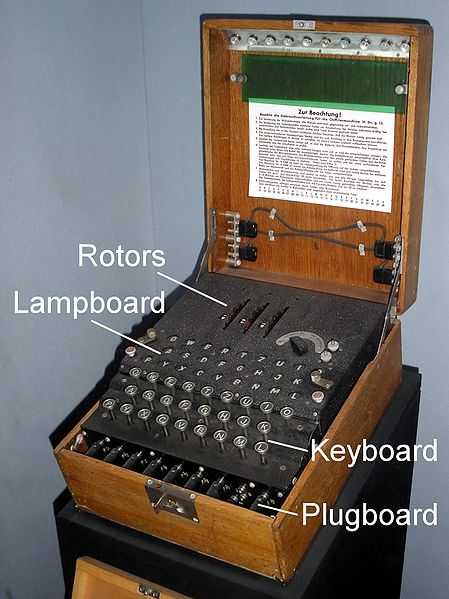
\includegraphics[width=0.45\textwidth]{images/main/enigma}
\end{center}
%
\begin{itemize}
\item Ένα πληκτρολόγιο αποκλειστικά με γράμματα (οι αριθμοί στέλνονταν ως κείμενο, το ίδιο και τα σημεία στίξης).
\item Ένα panel με λαμπάκια (όχι LEDs, μη το τρέχετε, οι ημιαγωγοί δεν είχαν βρεθεί ακόμα!) τα οποία φωτίζουν αντίστοιχα γράμματα. Γνωστό και ως lampboard.
\item Ενα μπροστινό panel με καλώδια/βύσματα (plugboard) το οποίο είναι προαιρετικό. Στην απλή εκδοχή (για χρήση σε επιχειρήσεις) το plugboard δεν υπάρχει, το διαθέτουν όμως όλες οι μηχανές στρατιωτικής χρήσης.
\item Ένα χώρο όπου τοποθετούνται τρεις (τουλάχιστον) περιστρεφόμενοι ρότορες (rotors) και ένας ανακλαστήρας (reflector) για τα οποία θα μιλήσουμε αναλυτικά.
\end{itemize}

Ο τρόπος που γενικά χρησιμοποιείται η μηχανή είναι ο εξής:

\begin{itemize}
\item Αρχικά τοποθετούνται τα βύσματα στο plugboard. Ουσιαστικά το plugboard κάνει ένα αρχικό ανακάτεμα των γραμμάτων. Για παράδειγμα, αν βάλετε ένα καλώδιο από το Α στο Ε, όταν πατάτε το γράμμα Α στο πληκτρολόγιο θα ενεργοποιείται το καλώδιο που κανονικά αντιστοιχεί στο γράμμα Ε. Αυτό ισχύει και ανάποδα (το Ε αντιστοιχεί στο Α). Το ενδιαφέρον είναι ότι plugboard λειτουργεί και κατά την επιστροφή του σήματος προς το lampboard (γίνεται ανακάτεμα και της εξόδου). Το plugboard διαθέτει 10 καλώδια και δεν είναι υποχρεωτικό να χρησιμοποιηθούν όλα. Όπου δεν υπάρχει καλώδιο, το γράμμα αντιστοιχίζεται στον εαυτό του. Για την αρχική μας έκδοση θα παραλείψουμε εντελώς το plugboard. Θεωρήστε λοιπόν ότι δεν υπάρχει και θα επανέλθουμε σε αυτό αργότερα.
\item Οι ρότορες μπορούν να περιστραφούν χειροκίνητα και να τοποθετηθούν σε κάποιες αρχικές θέσεις, που προφανώς έχουν συμφωνηθεί από πριν. Οι ρότορες περιστρέφονται επίσης κατά τη διάρκεια της κρυπτογράφησης με συγκεκριμένο τρόπο που θα δούμε παρακάτω.
\item Ο χειριστής γράφει το μήνυμα του γράμμα – γράμμα και σημειώνει σε κάθε πλήκτρο ποιο λαμπάκι του lampboard ανάβει.
\item Το κρυπτογραφημένο μήνυμα αποστέλλεται με κάποιο ενδεχομένως μη-ασφαλή τρόπο (π.χ. ασύρματο) και ο παραλήπτης, έχοντας θέσει στη μηχανή του τις ίδιες ακριβώς αρχικές ρυθμίσεις, το πληκτρολογεί και σημειώνει ποια λαμπάκια ανάβουν. Το μήνυμα έχει αποκρυπτογραφηθεί.
\end{itemize}

Τα πράγματα είναι ακόμα πιο πολύπλοκα στην πραγματικότητα:

\begin{itemize}
\item Οι ρότορες είναι αφαιρούμενοι και μπορούν να τοποθετηθούν διαφορετικά είδη (rotor types) και με διαφορετική σειρά.
\item Ο ανακλαστήρας είναι επίσης αφαιρούμενος και διατίθεται σε διάφορους τύπους.
\item Εκτός από την μεταβλητή αρχική θέση, οι ρότορες διαθέτουν ακόμα μια εσωτερική ρύθμιση που ουσιαστικά μετατοπίζει την κρυπτογράφηση, γνωστή ως ring setting.
\end{itemize}

Μπορείτε να δείτε εδώ μια πολύ καλή περιγραφή και επίδειξη της λειτουργίας της μηχανής Enigma: \url{http://youtu.be/G2_Q9FoD-oQ} 

Το μεγάλο ατού της μηχανής είναι τα κινούμενα μέρη της: οι ρότορες. Σε πρώτη λοιπόν φάση θα δούμε πως είναι φτιαγμένος ένας ρότορας και πως κρυπτογραφεί. Και φυσικά, πως θα τον εξομοιώσουμε σε python.

\subsection{Ρότορας: Η Ψυχή του Enigma}

Είναι ένα εξαιρετικά απλό εξάρτημα αλλά και ιδιοφυές ταυτόχρονα. Φανταστείτε τον ρότορα σαν ένα κύλινδρο με 26 επαφές σε κάθε βάση, κυκλικά τοποθετημένες όπως φαίνεται στο σχήμα μας. Οι επαφές αυτές αποτελούν την είσοδο και έξοδο του ρότορα. Ας θεωρήσουμε τον κύλινδρο που βρίσκεται στο δεξιό άκρο της μηχανής μας. Οι επαφές στη δεξιά του βάση συνδέονται με το πληκτρολόγιο και οι αριστερές με τον επόμενο (μεσαίο κύλινδρο).  Όμως μη βιαστείτε να χωρίσετε τις επαφές σε εισόδους και εξόδους, καθώς οι ίδιες επαφές χρησιμοποιούνται και με την αντίστροφη κατεύθυνση για να ενεργοποιήσουν τα λαμπάκια του lampboard.

\begin{center}
  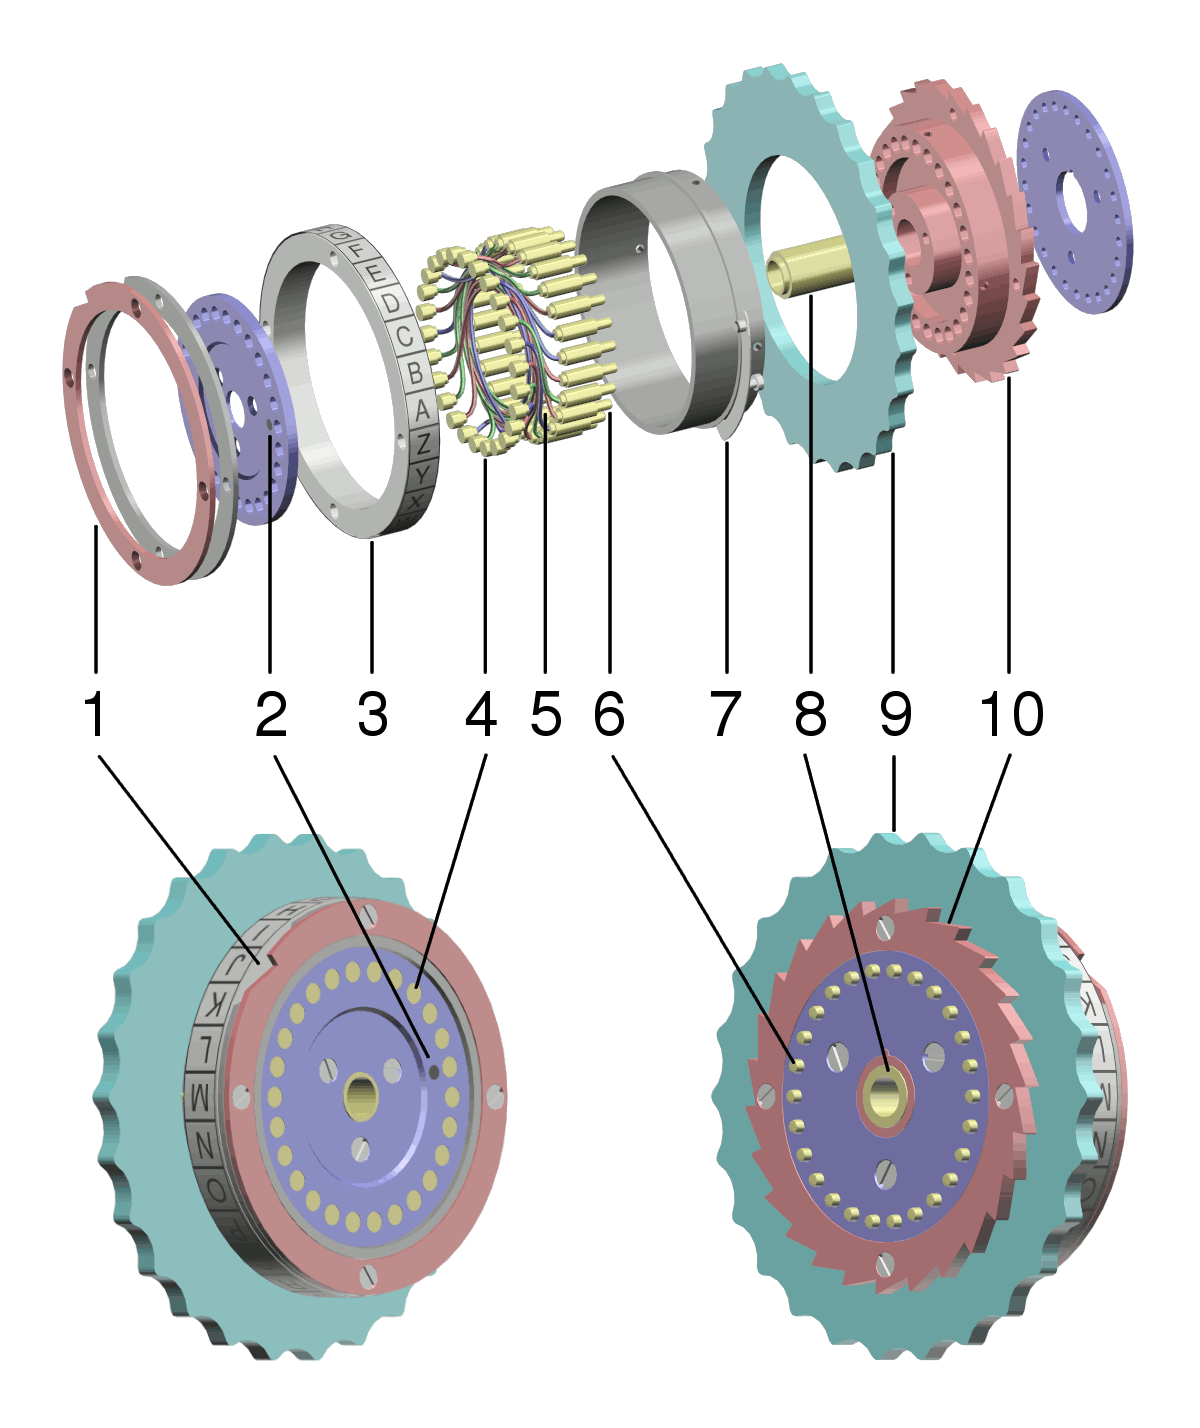
\includegraphics[width=0.6\textwidth]{images/main/rotors}
\end{center}

Τι περιέχει μέσα του ένας ρότορας; Καλώδια που αντιστοιχούν τις δεξιές με τις αριστερές επαφές. Για να το δούμε καλύτερα, θα πρέπει να θεωρήσουμε μια επαφή του ρότορα ως την αρχή του, και θα την συμβολίσουμε με το “Α”. Αν πάρουμε ένα ρότορα τύπου ΙΙΙ, η καλωδίωση του είναι η παρακάτω:

\begin{center}
\begin{tabularx}{\textwidth}{|*{26}{>{\centering\arraybackslash}X|}}
\hline
A&B&C&D&E&F&G&H&I&J&K&L&M&N&O&P&Q&R&S&T&U&V&W&X&Y&Z\\
\hline
B&D&F&H&J&L&C&P&R&T&X&V&Z&N&Y&E&I&W&G&A&K&M&U&S&Q&O\\
\hline
\end{tabularx}
\end{center}

(Μπορείτε να δείτε όλες τις καλωδιώσεις για τους ρότορες τύπων Ι, ΙΙ, ΙΙ και άλλων εδώ: \url{https://en.wikipedia.org/wiki/Enigma_rotor_details})

Αν δώσουμε ρεύμα στην επαφή “Α”, θα βγει από την επαφή “Β”, αν δώσουμε στην επαφή “Η”, θα βγει από την επαφή “P”.

Ίσως τώρα να σκέφτεστε ότι το “Α” του πληκτρολογίου καταλήγει στο “Α” στη δεξιά βάση του δεξιού ρότορα. Όχι απαραίτητα! Βλέπετε μπορούμε να ξεκινήσουμε την κρυπτογράφηση θέτοντας εμείς όποια αρχική θέση θέλουμε στους ρότορες. Περιστρέφοντας λοιπόν το ρότορα ώστε να δείχνει στη θέση “Η”, το Α του πληκτρολογίου θα συνδέεται στο “Η”. 

Το καταπληκτικό όμως είναι ότι ο δεξιός ρότορας του Enigma περιστρέφεται κάθε φορά που πιέζουμε ένα πλήκτρο, και μάλιστα πριν γίνει η ηλεκτρική σύνδεση της κρυπτογράφησης του!

Έτσι, αν έχετε βάλει ως αρχική θέση το “J” και πιέσετε το “Α”, ο δεξιός ρότορας θα περιστραφεί πρώτα στη θέση “K” και αμέσως μετά θα συνδεθεί το ηλεκτρικό κύκλωμα πλήκτρο “Α” => Θέση “Κ”. Αν αμέσως μετά πιέσετε το “D”, ο ρότορας θα περιστραφεί πρώτα στη θέση “L”, και θα γίνει η σύνδεση πλήκτρο “D” => Θέση “O” (Αφού το “L” είναι τώρα η πρώτη επαφή, το “D” που πιέσατε θα συνδεθεί στην τέταρτη που είναι το “Ο”). Ακόμα και αν πιέσετε 10 φορές το πλήκτρο Α συνεχόμενα, θα πάρετε 10 διαφορετικές κρυπτογραφήσεις. Και αυτό με ένα μόνο ρότορα!

Η έξοδος του δεξιού ρότορα πηγαίνει στο μεσαίο, και του μεσαίου στον αριστερό οπότε φανταστείτε ότι η διαδικασία “ανακατέματος” των γραμμάτων επαναλαμβάνεται άλλες δύο φορές! Και δεν τελειώσαμε. Βλέπετε, κάθε ρότορας έχει μια εγκοπή (η θέση της εξαρτάται από τον τύπο του) που ενεργοποιεί τον επόμενο. Ο δεξιός ρότορας περιστρέφεται κάθε φορά που πιέζουμε ένα πλήκτρο. Όταν φτάσει στην εγκοπή του, περιστρέφει το μεσαίο ρότορα κατά μια θέση. Και το ίδιο γίνεται με το μεσαίο: στην εγκοπή του περιστρέφει τον αριστερό.

Όταν το ρεύμα φτάσει στην αριστερή βάση του αριστερού ρότορα, εισέρχεται στον ανακλαστήρα. Ο ανακλαστήρας είναι ένα πολύ απλό εξάρτημα το οποίο έχει μόνο μια ενεργή βάση με 26 επαφές τις οποίες ενώνει ανά ζεύγη. Τα τρία βασικά είδη ανακλαστήρων είναι τα Α,B και C. Αν πάρουμε ένα τύπου Β και του δώσουμε ρεύμα στην επαφή “Α”, θα μας το επιστρέψει στην επαφή “Υ”. Από εκεί το ρεύμα θα κινηθεί αντίστροφα μέσα στους ρότορες μας μέχρι να φτάσει στο λαμπάκι που θα ενεργοποιηθεί στο lampboard. 

\subsection{Ρότορες σε Λειτουργία}

Πιέζοντας το “Α” στο πληκτρολόγιο, το ρεύμα διέρχεται από την πρώτη επαφή του δεξιού ρότορα, κινείται μέσα από τις καλωδιώσεις των άλλων δύο και ανακλάται από το reflector. Ακολουθεί αντίστροφη πορεία και ανάβει το λαμπάκι “G”. Πιέζοντας το “Α” για δεύτερη φορά, το αποτέλεσμα είναι διαφορετικό καθώς ο δεξιός ρότορας περιστρέφεται αλλάζοντας τη διαδρομή του ρεύματος (πηγή: wikipedia).
%
\begin{center}
  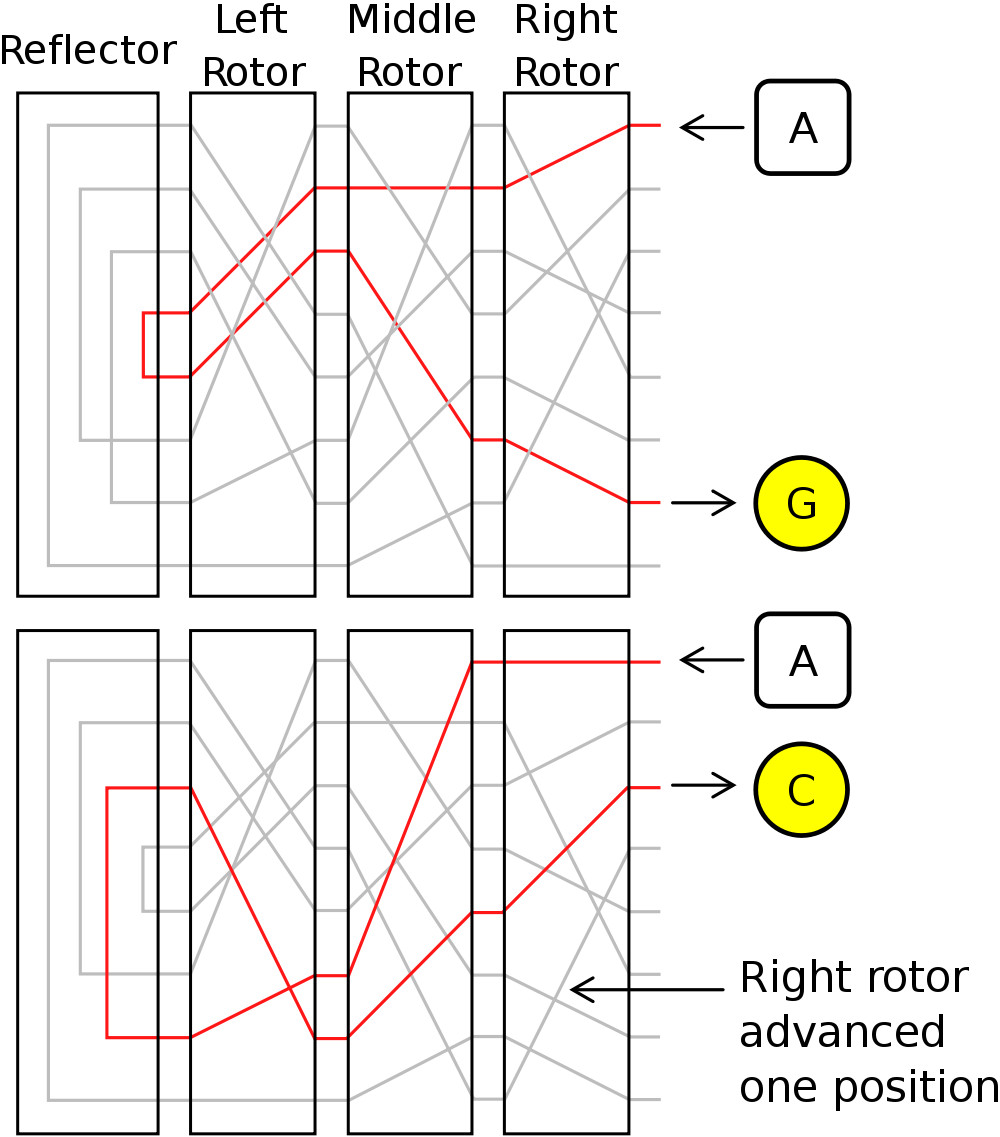
\includegraphics[width=0.8\textwidth]{images/main/rotor-work}
\end{center}
%

\subsection{Εξομοίωση Enigma  – Πρώτη απόπειρα}

Θα δημιουργήσουμε την απλούστερη δυνατή μηχανή Enigma, που  περιέχει μόνο ένα δεξιό ρότορα τύπου ΙΙΙ και ένα ανακλαστήρα τύπου Β. Σίγουρα δεν είναι ασφαλής, αλλά είναι μια αρχή για να προχωρήσουμε.

Φυσικά, θα χρησιμοποιήσουμε κλάσεις για να περιγράψουμε το ρότορα και τον ανακλαστήρα.

Ας ξεκινήσουμε από τον ανακλαστήρα. Περιέχει μια απλή λίστα με αντιστοιχίες ακροδεκτών. Στην κλάση μας προβλέψαμε τα δύο πιο συνηθισμένα είδη ανακλαστήρων, τα τύπου “Β” και τύπου “C” - η μόνη τους διαφορά είναι οι αντιστοιχίες:

\begin{minted}[bgcolor=bg, linenos, frame=lines, framesep=10pt]{python}
class Reflector(object):
    def __init__(self, type='B'):
        self.type = type
        if self.type == 'B':
            self.reflection_table = [24, 17, 20, 7, 16, 18, 11,
                                      3, 15, 23, 13, 6, 14, 10,
                                     12, 8, 4, 1, 5, 25, 2, 22,
                                     21, 9, 0, 19]
        else:
            self.reflection_table = [5, 21, 15, 9,  8,  0, 14, 24,
                                     4, 3,  17, 25, 23, 13, 6, 2,
                                     19, 10, 20, 16, 18, 1,
                                     13, 12, 7, 11] 
                
    def reflect(self, position):
        if position >=0 and position <=25:
            return self.reflection_table[position]
\end{minted}

Προφανώς η μόνη λειτουργία που εκτελεί αυτό το απλό εξάρτημα είναι η reflect. Για παράδειγμα:

\begin{minted}[bgcolor=bg,  frame=lines, framesep=10pt]{python}
thereflector = Reflector( “B”)
output = thereflector(0)
\end{minted}

Εδώ ζητάμε από τον ανακλαστήρα την\ldots ανάκλαση της επαφής 0, που αντιστοιχεί στο “Α” και το αποτέλεσμα θα είναι 24, που αντιστοιχεί στο “Y”.

Και πάμε στο ρότορα. Οι δυο βασικές του λειτουργίες είναι:

\begin{itemize}
\item \textbf{cipher:} Όταν ο ρότορας δέχεται ηλεκτρικό σήμα σε ένα ακροδέκτη στη δεξιά του βάση, το μεταδίδει σε ένα ακροδέκτη της αριστερής, σύμφωνα πάντα με μια λίστα που δίνει τις αντιστοιχίες ακροδεκτών.

\item \textbf{reflectCipher:} Αντίστροφη κρυπτογράφηση: όταν ο ρότορας δέχεται ηλεκτρικό σήμα σε ακροδέκτη της αριστερής βάσης, το μεταδίδει σε ακροδέκτη της δεξιάς, χρησιμοποιώντας την ίδια λίστα με πριν αλλά ανάστροφα!
\end{itemize}

Όμως έχει και άλλες ιδιότητες:

\begin{itemize}
\item \textbf{rotate:} Ο ρότορας περιστρέφεται κατά τη διαδικασία κρυπτογράφησης. Αν πρόκειται για το δεξιότερο ρότορα, περιστρέφεται σε κάθε πίεση πλήκτρου και πριν γίνουν οι ηλεκτρικές συνδέσεις.
\item Ο ρότορας τοποθετείται σε κάποια αρχική θέση με χειροκίνητη περιστροφή πριν ξεκινήσει η διαδικασία της κρυπτογράφησης.
\item Τέλος, καλό είναι να μπορούμε να τον ρωτήσουμε σε ποια θέση βρίσκεται.
\end{itemize}

\begin{minted}[bgcolor=bg, linenos, frame=lines, framesep=10pt]{python}
class Rotor(object):
    def __init__(self, startposition,placement):
       self.letter_ring = [ 'A', 'B', 'C', 'D', 'E',
                        'F', 'G', 'H', 'I', 'J',
                        'K', 'L', 'M', 'N', 'O',
                        'P', 'Q', 'R', 'S', 'T',
                        'U', 'V', 'W', 'X', 'Y', 'Z']
       self.placement = placement
\end{minted}

Το letter\_ring είναι ο δακτύλιος με τα γράμματα που μας επιτρέπει να βλέπουμε μεταξύ άλλων σε ποια αρχική θέση έχουμε τοποθετήσει το ρότορα μας. Μια τυπική μηχανή Enigma έχει τρεις ρότορες και εδώ το placement δείχνει αν ο ρότορας μας είναι τοποθετημένος αριστερά (left), στη μέση (middle) ή δεξιά (right). Αν είναι δεξιά, περιστρέφεται αυτόματα σε κάθε πίεση πλήκτρου.

\begin{minted}[bgcolor=bg, frame=lines, framesep=10pt]{python}
       self.position = ord(startposition) – 65
\end{minted}

Τη θέση τη δίνουμε σε μορφή γράμματος, “Α” - “Ζ” αλλά τη μετατρέπουμε σε αριθμό από 0 – 25

\begin{minted}[bgcolor=bg, linenos, frame=lines, framesep=10pt]{python}
       for i in range(0, self.position):
           self.rotate()
\end{minted}

Περιστρέφουμε το ρότορα μια-μια θέση μέχρι να φτάσει στην αρχική θέση που δώσαμε. Δεν είναι αποδοτικό, αλλά μοιάζει πολύ στην original μηχανή!

Και εδώ βλέπουμε τη συνάρτηση που κάνει την περιστροφή, τόσο για να πάμε χειροκίνητα στην αρχική θέση όσο και κατά τη διάρκεια της κρυπτογράφησης. Λογικό είναι όταν ο ρότορας περιστραφεί μέχρι το “Z” (25), επιστρέφει στο “Α” (0):

\small
\begin{minted}[bgcolor=bg, linenos, frame=lines, framesep=10pt]{python}
    def rotate(self):
        self.position +=1
        if self.position == 26:
            self.position = 0
        self.connections = self.connections[1:] + self.connections[0:1]
        self.letter_ring = self.letter_ring[1:] + self.letter_ring[0:1]
\end{minted}
\normalsize

Το self.connections δεν το έχουμε δει ακόμα, αλλά είναι η λίστα που περιέχει τις αντιστοιχίες των ακροδεκτών. Προσέξτε τι γίνεται στην περιστροφή. Ένας ρότορας στη θέση “Α”, έχει τις αντιστοιχίες που είδαμε παραπάνω:

\begin{center}
\begin{tabularx}{\textwidth}{|*{26}{>{\centering\arraybackslash}X|}}
\hline
A&B&C&D&E&F&G&H&I&J&K&L&M&N&O&P&Q&R&S&T&U&V&W&X&Y&Z\\
\hline
B&D&F&H&J&L&C&P&R&T&X&V&Z&N&Y&E&I&W&G&A&K&M&U&S&Q&O\\
\hline
\end{tabularx}
\end{center}

Ο ακροδέκτης μηδέν, είναι ο “Α”. Όταν ο ρότορας περιστραφεί μια θέση:	

\begin{center}
\begin{tabularx}{\textwidth}{|*{26}{>{\centering\arraybackslash}X|}}
\hline
B&C&D&E&F&G&H&I&J&K&L&M&N&O&P&Q&R&S&T&U&V&W&X&Y&Z&A\\
\hline
D&F&H&J&L&C&P&R&T&X&V&Z&N&Y&E&I&W&G&A&K&M&U&S&Q&O&B\\
\hline
\end{tabularx}
\end{center}

Ο ακροδέκτης μηδέν είναι ο “Β”. Πρέπει να περιστρέψουμε ταυτόχρονα  τη λίστα με τα γράμματα (letter\_ring) και τις αντιστοιχίες (connection) το οποίο λόγω της Python γίνεται εξαιρετικά εύκολα:

\begin{minted}[bgcolor=bg, frame=lines, framesep=10pt]{python}
self.letter_ring = self.letter_ring[1:] + self.letter_ring[0:1]
\end{minted}

self.letter\_ring[1:] μας δίνει τη λίστα ξεκινώντας από το δεύτερο στοιχείο της και στην άκρη προσθέτουμε ξανά το πρώτο γράμμα self.letter\_ring[0:1].

Και πάμε στην κρυπτογράφηση από δεξιά προς αριστερά που είναι εύκολη:

\begin{minted}[bgcolor=bg, frame=lines, framesep=10pt]{python}
    def cipher(self, letter):
        if self.placement == 'Right':
            self.rotate()
\end{minted}

Αν ο ρότορας είναι ο δεξιός, τον περιστρέφουμε πριν κάνουμε οτιδήποτε.

\begin{minted}[bgcolor=bg, frame=lines, framesep=10pt]{python}
        inputletter = self.letter_ring[letter]
        outputletter = self.connections[letter]
\end{minted}

Το letter στην πραγματικότητα είναι ο αριθμός του ακροδέκτη που ενεργοποιείται. Έχει μια τιμή από 0-25. Στο inputletter και outputletter έχουμε τα αντίστοιχα γράμματα σύμφωνα με τις λίστες αντιστοιχιών. Όμως αυτό που πραγματικά μας ενδιαφέρει είναι σε ποιο ακροδέκτη της δεξιάς βάσης καταλήγει το σήμα εξόδου, γιατί και στον επόμενο ρότορα θα δώσουμε είσοδο με βάση τον αριθμό αυτό:

\begin{minted}[bgcolor=bg, frame=lines, framesep=10pt]{python}
        outputindex = self.letter_ring.index(outputletter)
\end{minted}

Τέλος επιστρέφουμε ότι υπολογίσαμε:

\begin{minted}[bgcolor=bg, frame=lines, framesep=10pt]{python}
        return (inputletter, outputletter, outputindex)
\end{minted}

Εντελώς αντίστοιχα έχουμε την αντίστροφη κρυπτογράφηση (από δεξιά προς αριστερά):

\begin{minted}[bgcolor=bg, linenos, frame=lines, framesep=10pt]{python}
    def reflectCipher(self, letter):
        inputletter = self.letter_ring[letter]
        outputindex = self.connections.index(inputletter)
        outputletter = self.letter_ring[outputindex]
        return (inputletter, outputletter, outputindex)
\end{minted}

Όλο το παραπάνω ήταν φυσικά ένα superclass που καλύπτει κάθε πιθανό τύπο ρότορα. Αλλά για να φτιάξουμε ένα type III Rotor, δεν χρειαζόμαστε τίποτα άλλο από τη λίστα αντιστοιχιών:

\begin{minted}[bgcolor=bg, linenos, frame=lines, framesep=10pt]{python}
class RotorIII(Rotor):
    def __init__(self, startposition,placement='Right'):
        self.connections  = ['B','D','F','H','J','L','C',
                             'P','R','T','X','V','Z','N',
                             'Y','E','I','W','G','A','K',
                             'M','U','S','Q','O']

        super(RotorIII,self).__init__(startposition,placement)
\end{minted}

Το πρόγραμμα είναι το \textbf{enigma-simple.py}. Δείτε το αποτέλεσμα που έχει για την λέξη HELLO. Δοκιμάστε να δώσετε το αποτέλεσμα σαν είσοδο για να βεβαιωθείτε ότι κάνει αποκρυπτογράφηση. Δοκιμάστε να δώσετε πολλαπλές φορές το ίδιο γράμμα. Τι θα γίνει αν προσπαθήσετε να κρυπτογραφήσετε ένα string από 26 “Α”; Προκύπτει ποτέ το “Α” στην έξοδο; Όχι! Μόλις ανακαλύψατε ένα βασικό πρόβλημα του Enigma: ένα γράμμα δεν κρυπτογραφείται ποτέ στον εαυτό του. Και αυτό φίλοι μου ήταν αρκετό για να σπάσει η κρυπτογράφηση!

\subsection{Plugboard}

Το σύστημα αυτό με τα καλώδια βρίσκεται στο εμπρός μέρος της μηχανής. Διατίθενται 10 ζεύγη καλωδίων που ενώνουν γράμματα μεταξύ τους. Εδώ βλέπουμε δύο μόνο συνδέσεις. Αν κάπου δεν υπάρχει καλώδιο το γράμμα απλά αντιστοιχίζεται στο εαυτό του (πηγή: wikipedia).
%
\begin{center}
  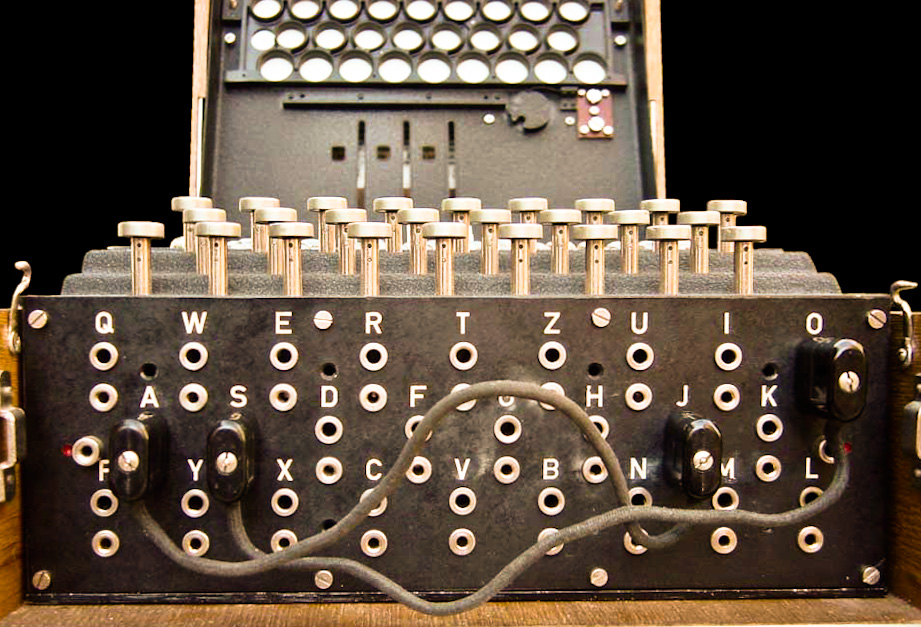
\includegraphics[width=0.7\textwidth]{images/main/plugboard}
\end{center}
%
\section{The Enigma Project -- Mέρος II}

Στο προηγούμενο μέρος ξεκινήσαμε την εξομοίωση της θρυλικής ηλεκτρομηχανικής συσκευής κρυπτογράφησης Enigma, κάνοντας την πρώτη μας απόπειρα για την απλούστερη υλοποίηση: μια μηχανή με ένα ρότορα και ένα ανακλαστήρα. Σε python φυσικά! Ήδη από την πρώτη αυτή υλοποίηση διαπιστώσαμε ένα σοβαρό μειονέκτημα της μηχανής (το οποίο σας διαβεβαιώνουμε, δεν διορθώνεται όσους ρότορες και αν βάλετε): Ένα γράμμα δεν κρυπτογραφείται ποτέ στον εαυτό του! Ίσως φαίνεται  λεπτομέρεια, όμως κάποιες τέτοιες φαινομενικά ασήμαντες διαπιστώσεις προκαλούν τελικά την κατάρρευση των καλύτερων συστημάτων κρυπτογράφησης. 

Καλό θα ήταν λοιπόν να δούμε:

\begin{itemize}
\item Γιατί συμβαίνει το παραπάνω; Γιατί η μηχανή μας (και ευτυχώς, όχι μόνο η δικιά μας!) είναι ανίκανη να αντιστοιχίσει μερικές φορές το “Α” στον εαυτό του;
\item Πως μπορεί κάποιος να επιτεθεί στην Enigma γνωρίζοντας το παραπάνω ελάττωμα;
\end{itemize}

Αν παρακολουθήσατε τα video του numberphile που σας προτείναμε (και σιγά που δεν τα παρακολουθήσατε δηλαδή, από δω βλέπω τα κόκκινα από το ξενύχτι  μάτια σας) θα είδατε τον τρόπο με τον οποίο ξεκινά η επίθεση στο Enigma:

\begin{itemize}
\item Πρέπει να γνωρίζουμε ή να μπορούμε να υποθέσουμε ένα μικρό κομμάτι cleartext που μεταδίδεται. Μα θα μου πείτε, αν γνωρίζουμε το cleartext γιατί να μπούμε στη διαδικασία της αποκρυπτογράφησης. Προσέξτε, όχι όλο το cleartext!
\end{itemize}

Σε ένα κρυπτογραφημένο μήνυμα, σχεδόν μοιραίο είναι ότι θα υπάρχει ένα κομμάτι τυποποιημένου, προβλέψιμου κειμένου το οποίο θα βρίσκεται μέσα του. Δεν ξέρουμε που, αλλά μπορούμε με ασφάλεια να πούμε ότι θα υπάρχει σε κάθε μήνυμα και θα είναι κρυπτογραφημένο με τον ίδιο ακριβώς τρόπο (τις ίδιες ρυθμίσεις) όπως και το υπόλοιπο σημαντικό κείμενο. Για παράδειγμα, στην επικοινωνία των Γερμανών με τα υποβρύχια τους είναι αναμενόμενο να βρούμε σε κάθε μήνυμα τη φράση “HEILHITLER”. Ή ίσως το πρωινό τους μήνυμα να περιέχει το δελτίο καιρού οπότε ψάχνουμε τη λέξη “WETTERBERICHT”.

Αν θέλετε να μεταφέρετε το παραπάνω στη σύγχρονη εποχή, ας υποθέσουμε ότι έχετε φτιάξει μια σύγχρονη μηχανή Enigma για να στέλνετε κρυπτογραφημένες εικόνες JPG. Θα τα πηγαίνατε μια χαρά – αλλά μάλλον θα πρέπει να συνειδητοποιήσετε ότι κάθε εικόνα JPG έχει μια τυποποιημένη επικεφαλίδα (header): Αν κάποιος ενδιάμεσος (κακόβουλος!) χρήστης ξέρει ότι μεταδίδετε εικόνες, μπορεί να ξεκινήσει ψάχνοντας για το κλειδί σας μέσα στο header: ξέρει το cleartext!

Στα μηνύματα όμως που στέλνονταν με το Enigma κατά τη διάρκεια του πολέμου, δεν γνωρίζαμε την ακριβή θέση που θα εμφανίζονταν το τυποποιημένο και προβλέψιμο cleartext μας. Φανταζόμαστε βέβαια ότι το “WETTERBERICHT” θα ήταν κάπου στην αρχή και το “HEILHITLER” κάπου στο τέλος – αλλά σε αντίθεση με την επικεφαλίδα του JPG – δεν μπορούμε να ξέρουμε τις ακριβείς θέσεις. Εδώ είναι που έρχεται το μειονέκτημα της Enigma που συζητήσαμε πριν: η μηχανή δεν κρυπτογραφεί ποτέ ένα γράμμα στον εαυτό του!

Αν λοιπόν ψάχνετε για τη λέξη “WETTERBERICHT” μέσα στο κρυπτόγραμμα μπορείτε να αποκλείσετε όλες τις περιπτώσεις όπου βλέπετε ένα γράμμα της να συμπίπτει με το κρυπτόγραμμα. Αν βρείτε μια πιθανή θέση μπορείτε να κάνετε υποθέσεις για την κρυπτογράφηση μέχρι να βρείτε – με την βοήθεια των μαθηματικών – τις αρχικές θέσεις κάθε ρότορα, δηλαδή το κλειδί!

Όλη αυτή τη δουλειά που σας περιγράψαμε παραπάνω, την έκανε ο γνωστός μας Alan Turing στο Bletchey Park – το κέντρο αποκρυπτογράφησης των Βρετανικών μυστικών υπηρεσιών στο Β' Παγκόσμιο πόλεμο. Και ναι, τα πάντα βασίστηκαν στα μαθηματικά. Αν δεν το έχετε λοιπόν δει ήδη, παρακολουθήστε το αντίστοιχο video του numberphile: \url{http://www.youtube.com/watch?v=V4V2bpZlqx8}.

Γιατί όμως η μηχανή Enigma έχει αυτό το μοιραίο ελάττωμα; Όπως θα διαβάσετε στο σχετικό σχήμα μας, το πρόβλημα οφείλεται στη χρήση του ανακλαστήρα.

\subsection{Εξομοίωση Enigma – Δεύτερη Απόπειρα}

Είχαμε σταματήσει στην εξομοίωση μιας μηχανής με ένα μόνο ρότορα και ένα ανακλαστήρα. Δεν είμαστε μακριά όμως από το να επιτύχουμε την πλήρη εξομοίωση της κανονικής μηχανής με τους τρεις ρότορες (ακόμα όμως χωρίς το περίφημο plugboard). Το μόνο που μένει είναι να ορίσουμε και τα άλλα είδη από ρότορες και να τους συνδέσουμε μεταξύ τους. Θα μπορούμε έπειτα να αντιμετωπίσουμε όλο το σύμπλεγμα των τριών rotors και του ανακλαστήρα σαν ένα ενιαίο μηχανισμό στον οποίο δίνουμε ως είσοδο ένα γράμμα και λαμβάνουμε στην έξοδο την κρυπτογραφημένη εκδοχή του. Θα βρείτε όλο το παρακάτω πρόγραμμα στο αρχείο \textbf{enigma-incomplete.py}. Όπως φαντάζεστε, θα δημιουργήσουμε μια κλάση RotorAssembly με τα παρακάτω χαρακτηριστικά:

\begin{itemize}
\item Μια συνάρτηση init στην οποία θα μπορούμε να δίνουμε και αρχικές θέσεις στους ρότορες του assembly.

\item Μια συνάρτηση cipher στην οποία θα δίνουμε το plaintext και θα μας επιστρέφει το ciphertext. Θα έχει επίσης “debug mode” στο οποίο θα δείχνει σε μορφή κειμένου (πίνακα) όλα τα ενδιάμεσα βήματα, όπως και το προηγούμενο απλουστευμένο μας πρόγραμμα.
\end{itemize}

Πριν όμως ξεκινήσουμε με το RotorAssembly, θα πρέπει να ορίσουμε τα άλλα δύο είδη από ρότορες που θα χρησιμοποιήσουμε, το Type II και το Type I. Κάτι αρκετά εύκολο, γιατί έχουμε ήδη το class και το μόνο που αλλάζει είναι η λίστα των αντιστοιχιών:

\small
\begin{minted}[bgcolor=bg, linenos, frame=lines, framesep=10pt]{python}
class RotorII(Rotor):
    def __init__(self,startposition,placement='Middle'):
        self.connections = ['A', 'J', 'D', 'K', 'S', 'I', 'R', 'U',
                            'X', 'B', 'L', 'H', 'W', 'T', 'M', 'C',
                            'Q', 'G', 'Z', 'N', 'P', 'Y', 'F', 'V',
                            'O', 'E' ]
        super(RotorII,self).__init__(startposition,placement)

class RotorI(Rotor):
    def __init__(self, startposition,placement='Left', ring_setting=1):
        self.connections  = [ 'E', 'K', 'M', 'F', 'L', 'G', 'D', 'Q',
                              'V', 'Z', 'N', 'T', 'O', 'W', 'Y', 'H',
                              'X', 'U', 'S', 'P', 'A', 'I', 'B', 'R',
                              'C', 'J' ]
        super(RotorI,self).__init__(startposition,placement)
\end{minted}
\normalsize

Και το απλό μας RotorAssembly:

\small
\begin{minted}[bgcolor=bg, linenos, frame=lines, framesep=10pt]{python}
class RotorAssembly(object):
    def __init__(self, startposition_left='Α', startposition_middle='Α',
        startposition_right='Α', reflectortype='B'):
        self.rotor_r = RotorIII(startposition_right, 'Right')
        self.rotor_m = RotorII(startposition_middle, 'Middle')
        self.rotor_l = RotorI(startposition_left, 'Left')
        self.reflector = Reflector(reflectortype)
\end{minted}
\normalsize

Παρατηρήστε ότι δίνουμε και κάποιες default τιμές στην init, ώστε κάποιος να μπορεί να δημιουργήσει ένα RotorAssembly  έτσι:

\begin{minted}[bgcolor=bg, frame=lines, framesep=10pt]{python}
assembly = RotorAssembly()
\end{minted}

οπότε οι τρεις ρότορες θα αρχικοποιηθούν στις θέσεις “Α”, “Α”, και\ldots “Α” και ο ανακλαστήρας θα είναι τύπου “B”. Ή μπορεί κάποιος να χρησιμοποιήσει τις δικές του τιμές:

\begin{minted}[bgcolor=bg, frame=lines, framesep=10pt]{python}
assembly = RotorAssembly('A', 'D', 'T', 'B')
\end{minted}

Όπως βλέπετε, το assembly μας περιέχει ένα ρότορα τύπου ΙΙΙ δεξιά, ένα τύπου ΙΙ στη μέση και ένα τύπου Ι αριστερά.  Φυσικά μπορείτε να αλλάξετε τις θέσεις τους αν θέλετε, αλλά μας βολεύει για να ελέγχουμε την κρυπτογράφηση μας με βάση κάποια άλλη εξομοίωση, όπως αυτή που θα βρείτε στο \url{http://enigmaco.de/enigma/} χωρίς να χρειαστεί να αλλάζουμε τα defaults.

Η συνάρτηση cipher απλά ενώνει τους ρότορες μεταξύ τους. Δείχνουμε εδώ ένα απλοποιημένο κομμάτι, και το υπόλοιπο θα το βρείτε στο αρχείο \textbf{enigma-incomplete.py}:

Θα αποθηκεύσουμε το ciphertext στην λίστα crypto:

\begin{minted}[bgcolor=bg, frame=lines, framesep=10pt]{python}
crypto = []
\end{minted}

Επεξεργαζόμαστε το μήνυμα γράμμα – γράμμα:

\begin{minted}[bgcolor=bg, frame=lines, framesep=10pt]{python}
for letter in themessage:
\end{minted}

Με τις παρακάτω τρεις κλήσεις κάνουμε την κανονική (από δεξιά προς τα αριστερά) κρυπτογράφηση στους τρεις ρότορες:

\footnotesize
\begin{minted}[bgcolor=bg, frame=lines, framesep=10pt]{python}
  (inputletter, outputletter, outpos) = self.rotor_r.cipher(ord(letter)-65)
  (inputletter, outputletter, outpos) = self.rotor_m.cipher(outpos)
  (inputletter, outputletter, outpos) = self.rotor_l.cipher(outpos)
\end{minted}
\normalsize

Φτάνουμε στον ανακλαστήρα:

\begin{minted}[bgcolor=bg, frame=lines, framesep=10pt]{python}
outpos = self.reflector.reflect(outpos)
\end{minted}

Επιστρέφουμε και κάνουμε την αντίστροφη κρυπτογράφηση (από αριστερά προς τα δεξιά):

\footnotesize
\begin{minted}[bgcolor=bg, frame=lines, framesep=10pt]{python}
  (inputletter, outputletter, outpos) = self.rotor_l.reflectCipher(outpos)
  (inputletter, outputletter, outpos) = self.rotor_m.reflectCipher(outpos)
  (inputletter, outputletter, outpos) = self.rotor_r.reflectCipher(outpos)
\end{minted}
\normalsize

Τελικά έχουμε το κρυπτογραφημένο μας γράμμα το οποίο τυπώνουμε και αποθηκεύουμε στη λίστα:

\begin{minted}[bgcolor=bg, frame=lines, framesep=10pt]{python}
  print chr(outpos+65)
  crypto.append(chr(outpos+65))
\end{minted}

Αν δοκιμάσετε τώρα να το τρέξετε με είσοδο “ΑΑΑΑΑ” (όπως σας το δίνουμε στο αρχείο) θα πάρετε την κρυπτογραφημένη έκδοση “BDZGO” η οποία όπως θα διαπιστώσετε αν διαβάσετε το άρθρο στην wikipedia (\url{http://en.wikipedia.org/wiki/Enigma_rotor_details}) ή στον εξομοιωτή που αναφέραμε, είναι το σωστό! Success. Αλλά μη βιάζεστε. Το ίδιο βιάζονταν και οι Γερμανοί και είδατε τι έπαθαν\ldots

Βλέπετε, στη μηχανή μας μόνο ο δεξιός ρότορας γυρίζει σε κάθε πάτημα πλήκτρου (σε κάθε γράμμα που του δίνουμε), ενώ η πραγματικότητα είναι ότι όταν ο δεξιός ρότορας φτάσει στην εγκοπή του (notch) θα πρέπει να περιστραφεί ο μεσαίος. Και αντίστοιχα, ο μεσαίος θα περιστρέψει τον αριστερό όταν φτάσει τη δική του εγκοπή. Ο αριστερός ρότορας – αν και διαθέτει εγκοπή – δεν επηρεάζει κάτι καθώς ο reflector είναι σταθερός.

Τότε γιατί το αποτέλεσμα είναι σωστό; Το μήνυμα μας είναι πολύ μικρό σε μέγεθος και οι αρχικές θέσεις στους ρότορες είναι τέτοιες που δεν ενεργοποιείται καμιά εγκοπή! Αν όμως βάλετε σαν αρχικές θέσεις το “Α”, “Α”, “Τ” για αριστερό, μεσαίο και δεξιό ρότορα αντίστοιχα, θα δείτε ότι η κρυπτογράφηση μας είναι λάθος: το πρόγραμμα μας, εκτός από το δεξιό, δεν ξέρει να περιστρέφει τους άλλους ρότορες!

Είναι ώρα να του διδάξουμε την περιστροφή και των άλλων rotors, μια διαδικασία γνωστή ως Enigma Steppings!

\subsection{Enigma Steppings}

Η αρχική υλοποίηση δε φαίνεται δύσκολη. Κάθε ρότορας έχει μια εγκοπή και όταν φτάσει εκεί κατά τη διάρκεια της περιστροφής του, δίνει μια ώθηση στον επόμενο ρότορα. Για τους δικούς μας τρεις τύπους ρότορα, οι εγκοπές είναι:

\begin{center}
\begin{tabular}{|c|c|c|}
\hline
\textbf{Ρότορας}&\textbf{Εγκοπή}&\textbf{Ενεργοποίηση επόμενου ρότορα}\\
\hline
Type III&V&Κατά την περιστροφή από V => W\\
\hline
Type II&E&Κατά την περιστροφή από Ε => F\\
\hline
Type I&Q&Κατά την περιστροφή από Q => R\\
\hline
\end{tabular}
\end{center}

Στους ρότορες φανταστείτε ότι οι εγκοπές βρίσκονται ανάμεσα στα γράμματα (π.χ. για τον Type III η εγκοπή βρίσκεται ανάμεσα στα V και W) αλλά φυσικά στο πρόγραμμα μας δεν μπορούμε να κάνουμε κάτι τέτοιο. Χρησιμοποιούμε τα γράμματα προορισμού για τις εγκοπές. Θα δείτε λοιπόν ότι σε κάθε ρότορα έχουμε προσθέσει μια γραμμή σαν τη παρακάτω:

\begin{minted}[bgcolor=bg, frame=lines, framesep=10pt]{python}
self.notch = 'W'
\end{minted}

Στο Rotor class έχουμε προσθέσει δύο συναρτήσεις που μας επιτρέπουν να δούμε αν είμαστε ακριβώς πριν το γράμμα που έχουμε ορίσει ως notch ή αν το έχουμε φτάσει:

\begin{minted}[bgcolor=bg, linenos, frame=lines, framesep=10pt]{python}
    def justBeforeNotch(self):
        if self.letter_ring[0] == chr(ord(self.notch)-1):
            return True
        else:
            return False

    def reachedNotch(self):
        if self.letter_ring[0] == self.notch:
            return True
        else:
            return False
\end{minted}

Και \emph{φαίνεται} (δώστε έμφαση στα πλάγια γράμματα) πως το μόνο που μένει είναι να φτιάξουμε λίγο το προηγούμενο μας κώδικα ώστε να ελέγχει πότε φτάνουν οι ρότορες στην εγκοπή για να ενεργοποιείται η περιστροφή του επόμενου ρότορα. Κάτι σαν το παρακάτω δηλαδή (το πλήρες πρόγραμμα είναι το \textbf{enigma-stepping1.py}):

\begin{minted}[bgcolor=bg, linenos, frame=lines, framesep=10pt]{python}
if self.rotor_r.reachedNotch():
    self.rotor_m.rotate()

if self.rotor_m.reachedNotch():
    self.rotor_l.rotate()
\end{minted}

Ωραία λοιπόν, εκτελέστε το πρόγραμμα \textbf{enigma-stepping1.py}. Σε αυτό έχουμε δώσει ως αρχικές τιμές στους ρότορες τις “A”, “A” και “Τ” και για μήνυμα τα γνωστά μας πέντε “Α”. Τι απάντηση πήρατε;

“AAAAA” => “BMUQO”

Γνωστοί για την ανυπομονησία σας, το δοκιμάζετε στην εξομοίωση enigmaco.de και βλέπετε ότι είναι σωστό. Success! αναφωνείτε για δεύτερη φορά. Πάλι βιάζεστε – τζάμπα τα πλάγια γράμματα δηλαδή. Δεν το πήρατε το hint;

Εντάξει λοιπόν, ας δοκιμάσουμε κάτι άλλο. Βάλτε σαν αρχικές θέσεις “A”, “D”, “T” και δοκιμάστε ξανά. Ο δικός μας εξομοιωτής δίνει:

“AAAAA” => “EEQEZ”

ενώ στο enigmaco.de θα πάρετε:

“AAAAA” => “EEQIB”

Καλά ξεκινάμε, αλλά κάτι χαλάει μετά! Τι; Οι αρχικές θέσεις που βάλαμε δεν ήταν και τόσο.. ε τυχαίες ας πούμε.  Και δείτε τι έγινε: όταν ο δεξιός ρότορας πέρασε από το “V” στο “W” περιστράφηκε (και σωστά) ο μεσαίος στη θέση “Ε”. Η θέση αυτή είναι ακριβώς πριν την εγκοπή του.

Τώρα το σωστό θα ήταν όταν ο δεξιός ρότορας κάνει μια ακόμα πλήρη περιστροφή και φτάσει ξανά στην εγκοπή του (V=>W), να περιστρέψει ξανά το μεσαίο ο οποίος (καθώς θα περνάει από το E=>F) θα περιστρέψει και τον αριστερό. Περίπου όπως περιστρέφονται τα ψηφία σε ένα οδόμετρο αυτοκινήτου. Αντί για αυτό τι γίνεται;

Όταν ο μεσαίος ρότορας φτάσει ακριβώς πριν την εγκοπή του, στο επόμενο πάτημα πλήκτρου περιστρέφεται ξανά χωρίς να ενεργοποιηθεί από το δεξιό!

Το φαινόμενο αυτό είναι γνωστό ως enigma double stepping και έχει φυσικά ως αποτέλεσμα την περαιτέρω εξασθένιση της κρυπτογράφησης!

Αν το Enigma το είχε φτιάξει η\ldots Microsoft, θα σας έλεγε ότι πρόκειται για\ldots feature. Εγώ σας διαβεβαιώνω ότι πρόκειται για bug! Ο τρόπος που λειτουργεί ο μηχανισμός (με τους μοχλούς, εγκοπές και λοιπά\ldots μηχανολογικά κόλπα) που μεταδίδει την κίνηση στους ρότορες προκαλεί και το double stepping.

Το θέμα είναι ότι αυτό το bug πρέπει να το περάσουμε και εμείς στο δικό μας κώδικα. Θέλουμε μια κανονική enigma, με τα προβλήματα της!

\subsection{Enigma Double Stepping}

Το πρόγραμμα μας είναι το \textbf{enigma-stepping2.py} και περιέχει τις παρακάτω αλλαγές:

\begin{minted}[bgcolor=bg, linenos, frame=lines, framesep=10pt]{python}
just_rotated = False
for letter in themessage:
  if self.rotor_m.justBeforeNotch():
    self.rotor_m.rotate()
    self.rotor_l.rotate()
    just_rotated = True
    if showoutput:
      print "DS"
  else:
    just_rotated = False
    if showoutput:
      print
\end{minted}

Αν ο μεσαίος ρότορας είναι ακριβώς πριν την εγκοπή, τον περιστρέφουμε άμεσα στο επόμενο πάτημα πλήκτρου. Γιατί το κάνουμε αυτό στην αρχή όμως και όχι μετά την περιστροφή του δεξιού ρότορα όπως θα ήταν πιο σωστό;

Κάποιος μπορεί να βάλει ως αρχική θέση “A”, “E”, “V”. Εδώ, ο δεξιός και ο μεσαίος ρότορας είναι ακριβώς πριν τις εγκοπές τους. Ξεκινώντας, ο δεξιός ρότορας θα περιστρέψει το μεσαίο, ο οποίος δεν πρέπει να περιστραφεί ξανά στο επόμενο πλήκτρο! Αν και βρίσκεται πριν την εγκοπή, τυχαίνει η περιστροφή του να συμπίπτει με τη φυσιολογική ώθηση που δέχεται από το δεξιό ρότορα. Δεν μπορώ να φανταστώ τι έπιναν όταν το κατασκεύαζαν αυτό το μηχάνημα!

Για την περίπτωση αυτή φυσικά πρέπει προσέξουμε να μη τον περιστρέψουμε ξανά παρακάτω:

\begin{minted}[bgcolor=bg, frame=lines, framesep=10pt]{python}
if self.rotor_r.reachedNotch() and not just_rotated:
  self.rotor_m.rotate()
\end{minted}

Δοκιμάστε τώρα αυτή την εκδοχή με τις αρχικές θέσεις που δώσαμε παραπάνω και επιβεβαιώστε τα αποτελέσματα. 

\subsection{Η Αδυναμία της Μηχανής}
%
\begin{center}
  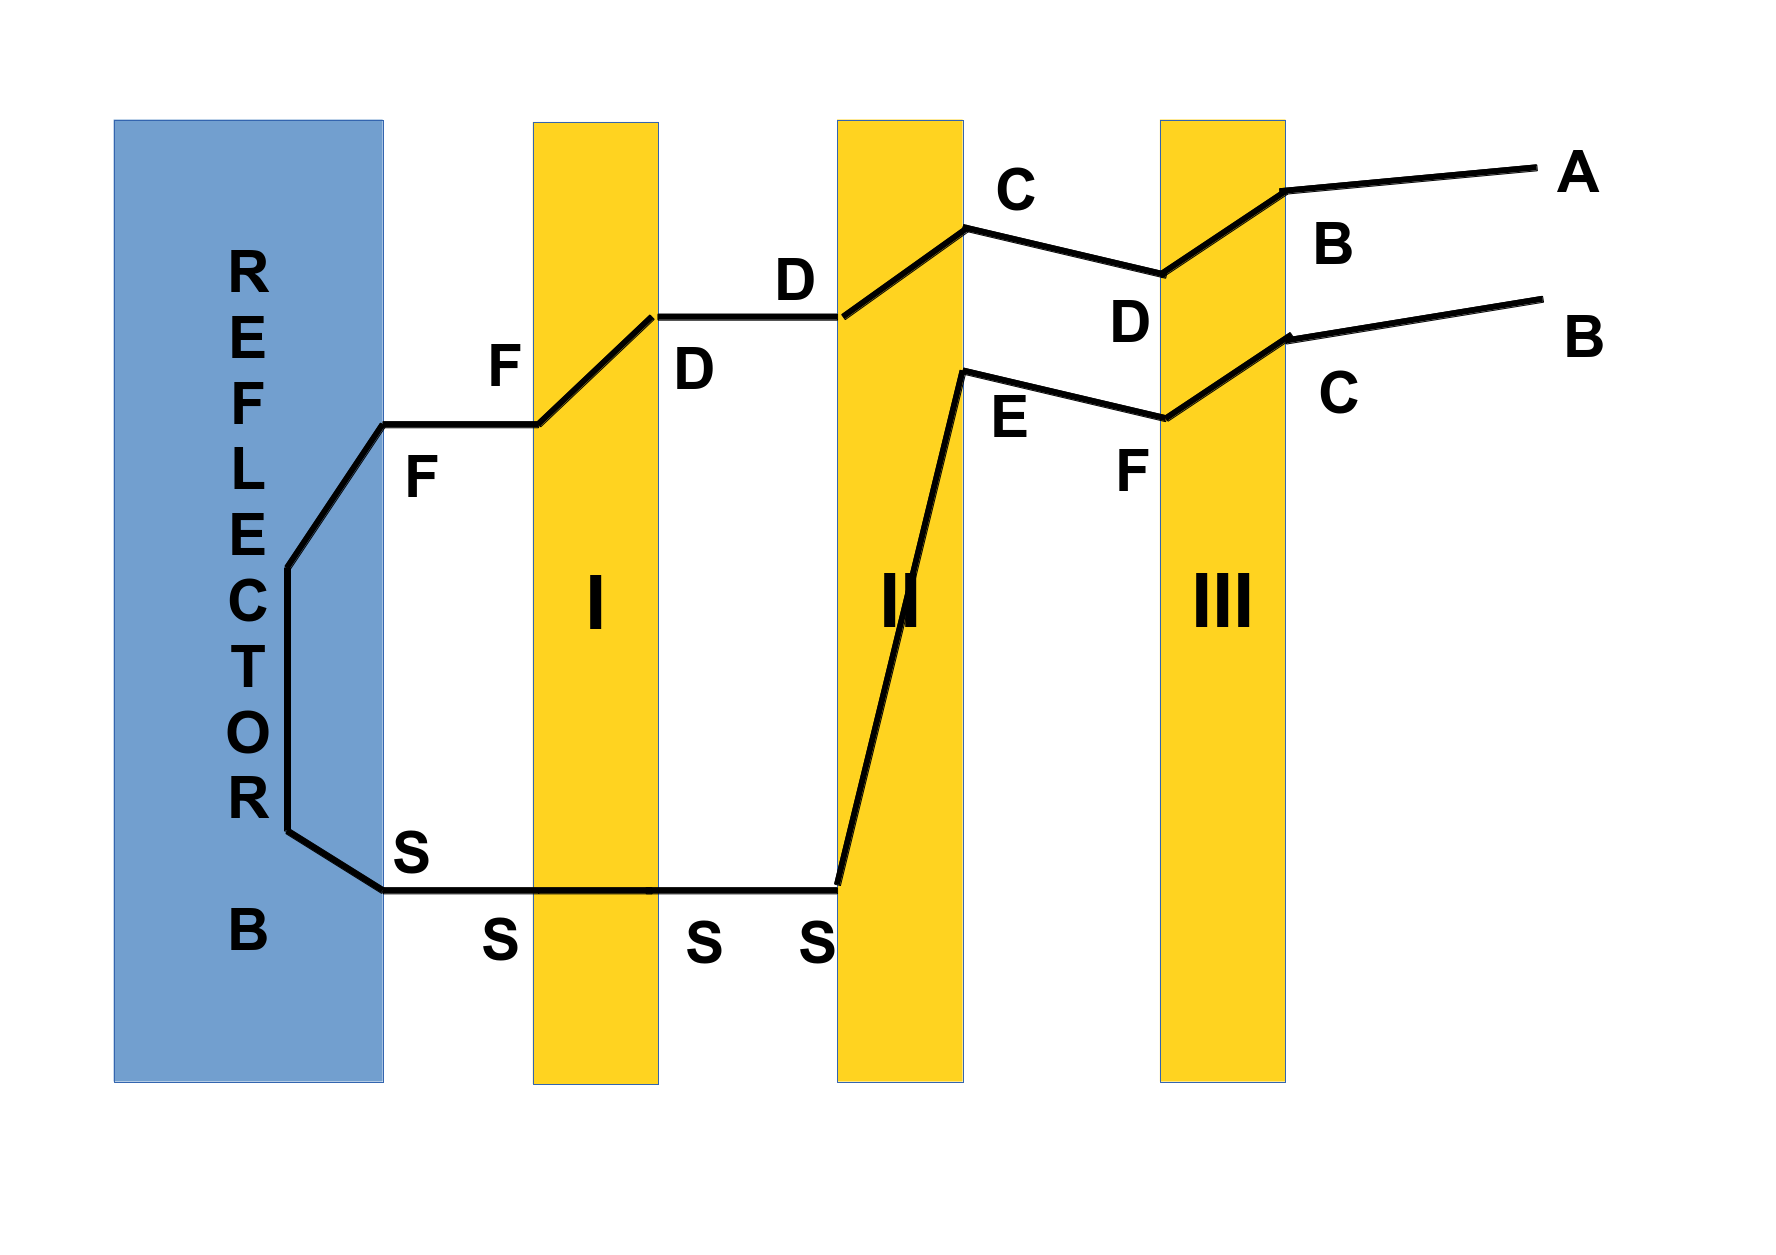
\includegraphics[width=0.7\textwidth]{images/main/flaw}
\end{center}
%
Γιατί αυτή η καταπληκτική μηχανή δεν μπορεί να κρυπτογραφήσει ένα γράμμα στον εαυτό του; Αν μπορούσε βέβαια, τα πράγματα θα ήταν πολύ πιο δύσκολα για τον Alan Turing και τους συνεργάτες του στο Bletchey Park. Για να καταλάβουμε το πρόβλημα ας παρακολουθήσουμε την κρυπτογράφηση ενός γράμματος σε μια μηχανή με ρότορες Ι, ΙΙ, ΙΙΙ, ανακλαστήρα τύπου Β και αρχικές θέσεις Α, Α, Α. Ο χειριστής πιέζει το γράμμα Α, ο δεξιός ρότορας περιστρέφεται και στην πραγματικότητα το Α συνδέεται  στη θέση Β. Από εκεί έχουμε την ακολουθία B=>D, C=>D, D=>F και F=>S από τον ανακλαστήρα. Δεν φαίνεται να υπάρχει κάτι που να εμποδίζει την αντιστοίχιση του Α στον εαυτό του μέχρι εδώ. Παρατηρήστε μάλιστα ότι σε δυο διαδοχικούς ρότορες έχουμε σαν έξοδο το ίδιο γράμμα, το D. Και αν δούμε και την αντίστροφη διαδρομή, ο ρότορας Ι έχει ξεκάθαρα αντιστοίχιση από S=>S. Τι χαλάει την συνταγή;

Για να μπορεί ένα γράμμα να αντιστοιχιστεί τελικά στον εαυτό του, θα πρέπει η μηχανή να έχει τη δυνατότητα να στείλει το γράμμα πίσω από την ίδια ακριβώς διαδρομή που προέρχεται. Αλλά αυτό είναι αδύνατον τη στιγμή που χρησιμοποιείται ανακλαστήρας που ενώνει πάντα δύο διαφορετικά σημεία (π.χ. το F=>S αλλά δεν θα μπορεί να ενώσει το F=>F αφού αυτό δεν είναι κύκλωμα!) Ακόμα και από ηλεκτρικής άποψης αν το εξετάσουμε δεν θα ήταν δυνατόν να κλείσουμε κύκλωμα αφού η διαδρομή επιστροφής θα ήταν ίδια με την αρχική και χρησιμοποιούμε τους ίδιους ρότορες και στις δύο κατευθύνσεις. Θα μπορούσαν λοιπόν οι σχεδιαστές κατ'αρχήν να έχουν εξασφαλίσει μια διαφορετική διαδρομή επιστροφής (ίσως μέσα από άλλους ρότορες) ώστε να μη συγκρούεται με την κανονική. Η χρήση του ανακλαστήρα και του ίδιου κυκλώματος για είσοδο – έξοδο κάνει αδύνατη την ισχυρότερη αυτή κρυπτογράφηση. Ας ευχαριστήσουμε τον κατασκευαστή για αυτό του το λάθος!
\newpage
\section{Εισαγωγή στο Arduino}

\begin{description}

\item [Τι είναι το Arduino;]
To arduino είναι ένας μικροελεγκτής, προσαρμοσμένος σε μια πλακέτα και έτοιμος προς χρήση.
\item[Μας φώτισες. Και τι είναι ένας μικροελεγκτής;]
Φανταστείτε το μικροελεγκτή σαν ένα τσιπάκι που περιέχει μέσα του ένα ολόκληρο μικρό υπολογιστή. Είναι ένας υπολογιστής ειδικού σκοπού: δεν θα τον χρησιμοποιήσετε για να γράψετε ένα κείμενο αλλά μπορείτε να τον προγραμματίσετε να ελέγχει άλλες συσκευές: να αναβοσβήνει φωτάκια (LED), να περιστρέφει κινητήρες κλπ.
\item[Που χρησιμοποιείται;]
Παντού γύρω μας, χωρίς συχνά να του δίνουμε σημασία. Σχεδόν όλες οι ηλεκτρονικές συσκευές που διαθέτετε έχουν τουλάχιστον ένα μέσα τους. Το touchpad στο laptop που γράφω τις σημειώσεις αυτή τη στιγμή ελέγχεται από ένα μικροελεγκτή: διαβάζει την επιφάνεια αφής και στέλνει τα αντίστοιχα δεδομένα στην κεντρική πλακέτα του υπολογιστή. Το ψυγείο σας, ο φούρνος μικροκυμάτων, το κινητό, η τηλεόραση, το αυτοκίνητο, ο διεθνής διαστημικός σταθμός και τα ρομποτάκια που στείλαμε στον Άρη είναι γεμάτα μικροελεγκτές.
\item[Σε τι διαφέρει από ένα κανονικό υπολογιστή;]
Σε αντίθεση με τον υπολογιστή που χρησιμοποιούμε για τις καθημερινές μας εργασίες, ένας μικροελεγκτής έχει τα παρακάτω χαρακτηριστικά και διαφορές:
%
\begin{itemize}
\item Δεν διαθέτει λειτουργικό σύστημα. Δεν πρόκειται να βάλετε Windows σε ένα μικροελεγκτή!
\item Τρέχει κάθε φορά ένα και μοναδικό πρόγραμμα που πρόκειται να γράψουμε εμείς και κάνει μια συγκεκριμένη λειτουργία.
\item Κάθε φορά που τον ενεργοποιούμε αυτόματα αρχίζει να εκτελεί το πρόγραμμα που του βάλαμε πριν. Το πρόγραμμα αποθηκεύεται μόνιμα μέσα στο ίδιο το κύκλωμα. Οι μικροελεγκτές δεν διαθέτουν σκληρούς δίσκους αλλά flash μνήμη (όπως το usb stick που έχετε στη τσέπη σας) και μια μικρή ποσότητα μνήμης RAM για χρήση από το πρόγραμμα.
\item Οι μικροελεγκτές συνήθως λειτουργούν με ελάχιστη ενέργεια. Οι περισσότεροι μπορούν να δουλέψουν για αρκετό διάστημα με μια μπαταρία ρολογιού. Πολλά μοντέλα διαθέτουν κατάσταση χαμηλής ενέργειας και παραμένουν σχεδόν σβηστά αν δεν χρειάζεται να κάνουν κάτι.
\item Οι μικροελεγκτές είναι συνήθως πολλοί φτηνότεροι από οποιοδήποτε υπολογιστή.
\item Διαθέτουν ακροδέκτες που μπορούμε να χρησιμοποιήσουμε ως ``εισόδους'' (για να συνδέσουμε αισθητήρες θερμοκρασίας, διακοπτάκια κλπ) και ``εξόδους'' που μπορούμε να συνδέσουμε μικρούς ηλεκτρικούς κινητήρες, LED ή ακόμα και μικρές οθόνες.
\end{itemize}

\item[Δηλ. το Arduino είναι ένας μικροελεγκτής;]

Μικροελεγκτής είναι μόνο το τσιπάκι. Αυτό από μόνο του δεν θα ήταν εύκολο να το κάνουμε κάτι: χρειαζόμαστε ένα τρόπο για να το προγραμματίσουμε (απαιτεί να το συνδέσουμε σε ένα κανονικό υπολογιστή) και κάποιο εύκολο σύστημα για να του συνδέσουμε έξτρα εξαρτήματα (LED, κινητήρες, διακοπτάκια κλπ). Αν και θα μπορούσαμε να ξεκινήσουμε από το μηδέν για να τα φτιάξουμε όλα αυτά, είναι πολύ πιο εύκολο να αγοράσουμε ένα σύστημα που να μας δίνει ένα μικροελεγκτή έτοιμο προς χρήση. Ένα τέτοιο σύστημα είναι το Arduino.

\item[Πόσο κοστίζει ένα Arduino; Που θα βρούμε;]

Ανάλογα με το μοντέλο κοστίζει μέχρι μερικές δεκάδες ευρώ. Το πιο συνηθισμένο μοντέλο είναι το Arduino Uno το οποίο στοιχίζει γύρω στα 10 ευρώ (και λιγότερο σε μεγάλες παραγγελίες από Κίνα!) Μεγαλύτερα μοντέλα μπορεί να κάνουν μέχρι και 50-60 ευρώ. Τα ακριβά μοντέλα διαθέτουν ταχύτερους μικροελεγκτές με περισσότερη μνήμη και είναι κατάλληλα για πολύ πιο πολύπλοκες εφαρμογές (έλεγχος πυραυλικών συστημάτων!)

Θα σας δώσω από ένα Arduino και μερικά ακόμα εξαρτήματα \textbf{στον καθένα σας} για να πάρετε σπίτι σας και να πειραματιστείτε. Στις σημειώσεις αυτές θα βρείτε προγραμματάκια για να παίξετε και να πειραματιστείτε. Η τελική μας εφαρμογή του Enigma θα χρησιμοποιήσει συνολικά τρεις μικροελεγκτές!

\item[Έχουμε δηλαδή δέκα Arduino; Όταν τελειώσει το Enigma τι θα τα κάνουμε;]

Δεκάξι, για να είμαι ακριβής :D
 
Όποιος μου αποδείξει ότι τον ενδιαφέρει και πρόκειται να συνεχίσει να το χρησιμοποιεί για να μαθαίνει, θα του το χαρίσω. Τα υπόλοιπα θα γίνουν δωρεά στο εργαστήριο ηλεκτρονικών και πληροφορικής του σχολείου
\end{description}

\item[Καμιά εικόνα;]

Ναι. Αυτό είναι το Arduino Uno (έχουμε 6):

-- diagram --

Και αυτό το Arduino Nano (έχουμε 10):

-- diagram --

\item[Πως συνδέουμε εξαρτήματα;]

Χρησιμοποιούμε τους ακροδέκτες που βλέπετε και συνδέουμε καλωδιάκια (jumper cables) τα οποιά καταλήγουν σε μια breadboard όπου φτιάχνουμε το υπόλοιπο κύκλωμα. Το Arduino Nano μπορεί να τοποθετηθεί το ίδιο απευθείας πάνω στη breadboard.

\item[Breadboard; Jumper cables;]

Breadboard είναι το παρακάτω εξάρτημα:

-- diagram --

Μας επιτρέπει να συνδέουμε και να ξεσυνδέουμε εξαρτήματα χωρίς να τα χαλάμε και τη χρησιμοποιούμε για να κάνουμε πειραματικές διατάξεις. Τα jumper cables χρησιμοποιούνται για να συνδέσουν τα εξαρτήματα μεταξύ τους.

Οι τρυπούλες στη breadboard ενώνονται μεταξύ τους κάθετα. Υπάρχει όμως ένα χώρισμα στη μέση.  Π.χ. το παρακάτω κύκλωμα δείχνει πως θα φτιάχναμε ένα κύκλωμα με ένα LED, μια αντίσταση και μια μπαταρία:

-- diagram --


\item[Αντίσταση;]

Είναι ένα βασικό εξάρτημα της ηλεκτρονικής -- χρειάζεται για να περιορίζει το ρεύμα --. Χωρίς αυτήν το LED μπορεί να καεί. Θα σας δώσω τις κατάλληλες αντιστάσεις για τα πειράματα σας και δεν χρειάζεται να μάθετε περισσότερες λεπτομέρειες (αν δεν θέλετε. Αν θέλετε εδώ είμαστε).

\subsection{Ελέγχοντας ένα LED με ένα Arduino}

Τώρα που είδατε πως μπορείτε να ενεργοποιήσετε ένα LED με μια μπαταρία, ας βάλουμε και το Arduino στο κύκλωμα μας. Εδώ είναι το παράδειγμα μας με το Arduino Nano:

-- diagram --

Θα θέλαμε να κάνουμε το LED να αναβοσβήνει χρησιμοποιώντας το μικροελεγκτή μας. Για το σκοπό αυτό, πρέπει να γράψουμε ένα μικρό πρόγραμμα.
Στο CD που σας δόθηκε υπάρχει ένα πρόγραμμα που πρέπει να εγκαταστήσετε στον υπολογιστή σας και λέγεται Arduino IDE.
Το πρόγραμμα υπάρχει στα έτοιμα παραδείγματα. Πηγαίνετε στο File -> Examples -> Basics -> Blink

-- photo --

Από το μενού Tools -> Board επιλέξτε Arduino Nano και από το μενού Tools -> Port την επιλογή COM που εμφανίζει (π.χ. COM4). Πριν εκτελεστεί ο κώδικας, θα πρέπει να μεταγλωττιστεί και να ελεγχθεί πιέζοντας το:

-- photo --

και τέλος να μεταφερθεί στο Arduino, πιέζοντας το:

-- photo --

Θα δείτε το LED να αναβοσβήνει. Εκτός από αυτό που έχουμε συνδέσει εμείς θα δείτε και ένα LED στην πλακέτα να αναβοσβήνει. Στην πραγματικότητα είναι συνδεμένα και τα δύο στην ίδια έξοδο (ψηφιακή έξοδος 13) οπότε αναβοσβήνουν μαζί.

Μπορείτε να μετατρέψετε το πρόγραμμα και το κύκλωμα ώστε να αναβοσβήνουν το LED αν το συνδέσετε στην έξοδο 12; Τι θα πρέπει να αλλάξετε; Μπορείτε να κάνετε το LED να αναβοσβήνει πιο γρήγορα;


\subsection{Πως δουλεύει το πρόγραμμα;}

 

\begin{itemize}
\item 
\end{document}
